\sectionauthor[Simon Blom; Sameh Mikhail]{Testing}
% The Testing section of your report is essential for demonstrating the effectiveness of your prototype under various conditions. This section is vital to prove not just that your design works, but how well it works, particularly in relation to the variable you've chosen to optimize. Your approach to testing should demonstrate a thorough, scientific method of evaluation, showcasing a deep understanding of your prototype's performance.
% \begin{itemize}
%     \item Testing Method: Clearly outline your testing methods, including the setup and conditions of the tests. Crucially, identify at least one key variable that you have chosen to optimize for in your design. This variable should be central to the performance and objectives of your prototype.
%     \item Results: Present the results of your tests in an organized and understandable manner. Utilize tables, graphs, and charts to effectively illustrate your findings, ensuring that they are directly related to the chosen variable for optimization and other tested parameters.
%     \item Analysis: Provide a critical analysis of your test results. Discuss the implications of the findings in relation to your project goals and the variable you aimed to optimize. Look for trends, patterns, or significant observations that emerge from the data and articulate what these mean for the effectiveness of your prototype.
% \end{itemize}

\subsection{Wind tunnel}
One of the important aspects that can be tested is the drag and lift in the air. It was tried to do a computational simulation on the wings and the plane, but due to unforeseen circumstances it was tackled in a different way. The Makerspace has a wind tunnel that was put to great use.

The wind tunnel setup allows for the precise measurement of aerodynamic forces acting on the wing. The fan generates a consistent airflow, simulating flight conditions, while the pressure sensors monitor the air pressure before and after the wing. This helps determine the pressure differential contributing to lift and drag.

The wing is mounted on a fixture designed to minimize interference with the airflow. The weight scales are calibrated to measure the forces in two directions: one aligned with the airflow (drag) and one perpendicular to it (lift). This configuration ensures accurate readings that reflect the wing's aerodynamic performance.

Before testing, a baseline measurement is taken with the wing absent to account for the drag induced by the apparatus itself. The wing is then mounted. Various angles of attack are tested to observe how the lift and drag vary with orientation. Data collected from the weight scales and pressure sensors are recorded and analyzed.

\begin{figure}[h]
    \centering
    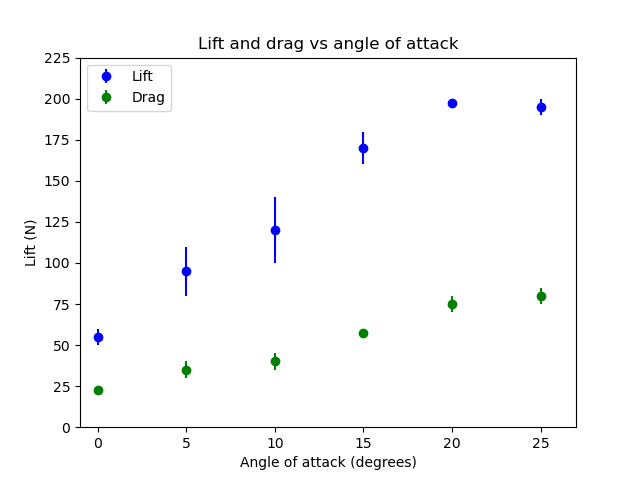
\includegraphics[width=0.5\linewidth]{images/windtunnel.png}
    \caption{Measurements of the lift and drag varying the angle of attack}
\end{figure}

\noindent and to make these results more valid, a linear fit based on the equations of motion was applied 

\begin{figure}[h]
    \centering
    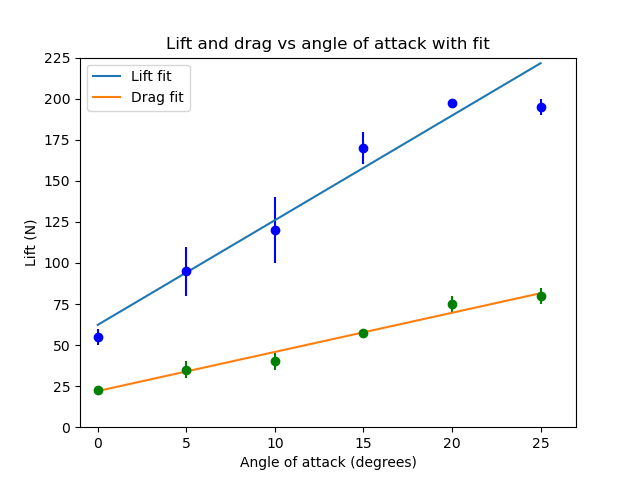
\includegraphics[width=0.5\linewidth]{images/windtunnel_fit.png}
    \caption{Fit of the measurements of the lift and drag varying the angle of attack}
\end{figure}

\noindent resulting in the equations for the lift and drag

\begin{equation}
    L = 6x + 62 \qquad \text{and} \qquad D = 2.4x + 22
\end{equation}
with $L$ and $D$ the weight of the lift and drag in terms of grams and $x$ the angle of attack of the wind. This is not an `infinite' linear relation: after 25 degrees the wing vibrated and changed angle so that the results after that became invalid.

One of the best indications if the results are valid is the so called reduced chi-squared $\chi_{\nu}^{2}$. The results are valid if the chi-squared is around the one. The first equation (of the lift) has a reduced chi-squared of 10 and the second equation (of the drag) has a reduced chi-squared of 0.7. If the reduced chi-squared is above one, like in this case, the errors might be to small. This is visible in the data: the first and last two point are too small and the fit does not go through the point or the error. A reduced chi-squared of 0.7 is very good, so that equation is valid. An argument for the validity of both functions is that when the angle is zero, the value for the function corresponds to the meassured value.

\subsection{Motor and prop thrust}
When the electrical circuit was fully assembled and soldered together, a test setup was constructed with tools available at this time around the Makerspace, as visible in Figure \ref{fig:Motor testing setup}. The brushless motor, the Pichler Boost 10, was clamped to a vice with an APC E 6x4 propellor attached. Then, this contraption was attached to a scale using Duck-tape and set to zero.

This was simultaneously the first time a wireless connection between the Ground Control Station (Simon's laptop) and parts of the Albatrone was attained. After changing a lot of parameters in the software, the motor's RPM was able to be fully controlled by the throttle stick on the remote.

The testing contraption was mounted on a few degrees angle because of the limits on the vice, the measured values will have a small margin of error. With full throttle, 393 grams of thrust was measured, which was within the expected margins of the calculated values using \cite{RCPlanes}. 

"In order to get reasonable climb and acceleration capabilities, the Static Thrust should be at least about 1/3 of the planes' weight." \cite{RCPlanes}. The weight of electronics used, were in on around 400 grams. This leaves 800 grams for the filament. This goal is expected to be attainable. Even if this 1/3 Static Thrust goal is not met, the drone should still be able to achieve stable flight, but with the catch of less maneuverability.

\begin{figure}[h]
     \centering
     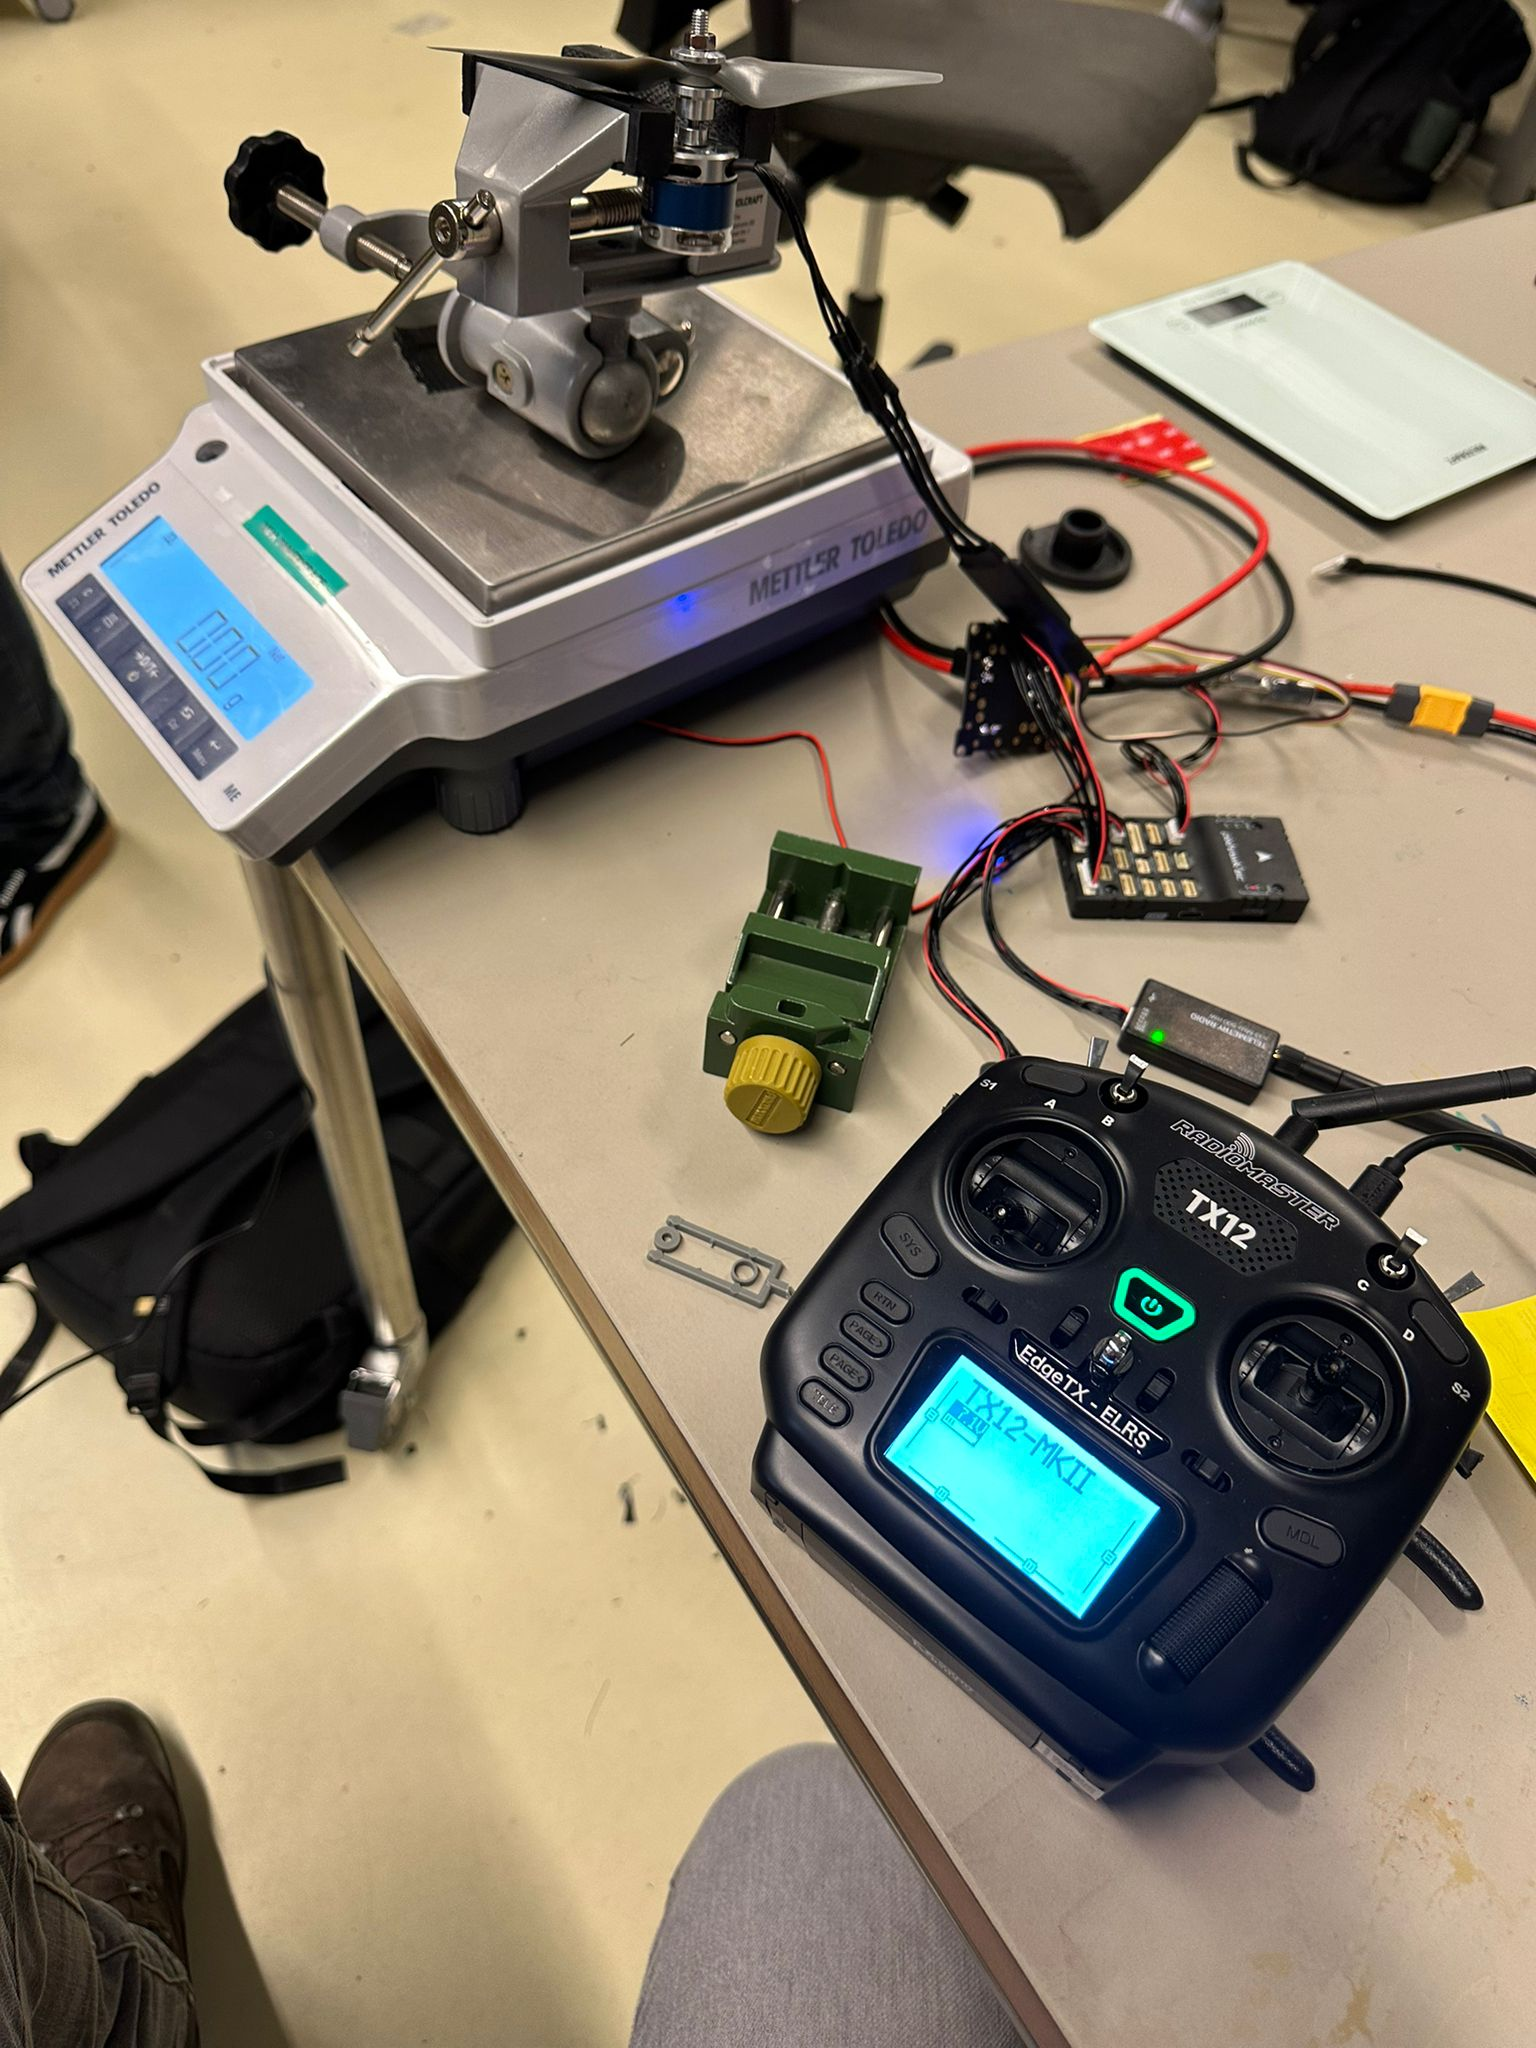
\includegraphics[width=0.5\linewidth]{images/Motor_test.jpg}
     \caption{The motor testing setup}
     \label{fig:Motor testing setup}
 \end{figure}

\subsection{Connection range}
Since the goal is to construct something that is able to fly, it is important to know the range from which this prototype can be controlled. As of writing this report, the RC controls of the airplane is run through the telemetry link as there is no need to extended the range of a seperate RC link via ELRS \cite{ELRS} for this prototype. 

The Telemetry link consists of 2 100mW Holybro SiK Telemetry V3 Radios  of the 433MHz variant. One is plugged into the Ground Control Station, see Figure \ref{fig:range}, and the other is plugged into the Pixhawk 6C, the Flight Controller chosen for this prototype. This test was performed on the Science Park Campus, so the performance over the resulting range is expected to not be optimal due to signal interference. Full control of the attached servo and motor was attained, until around 200m, with stutters until 209m measured with GPS, see Figure \ref{fig:range}.

\begin{figure}
\centering
\begin{subfigure}{.5\textwidth}
  \centering
  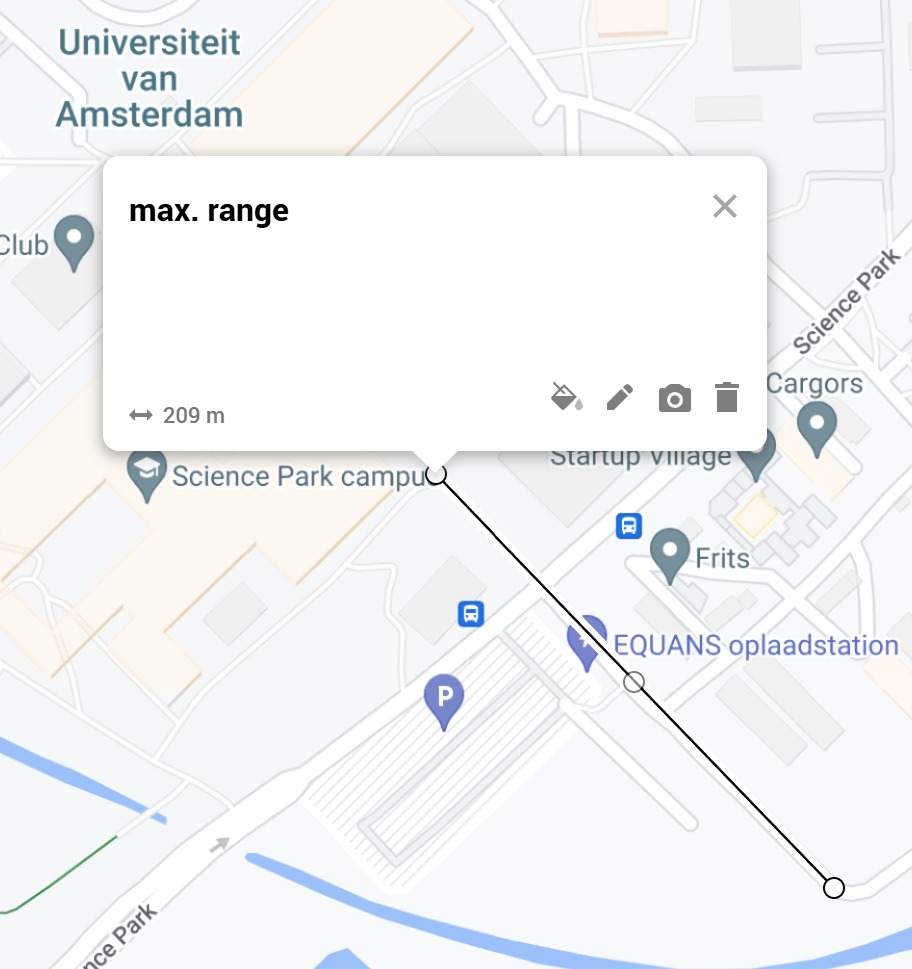
\includegraphics[width=.8\linewidth]{images/range_test.jpg}
  \label{fig:maxrange}
\end{subfigure}%
\begin{subfigure}{.5\textwidth}
  \centering
  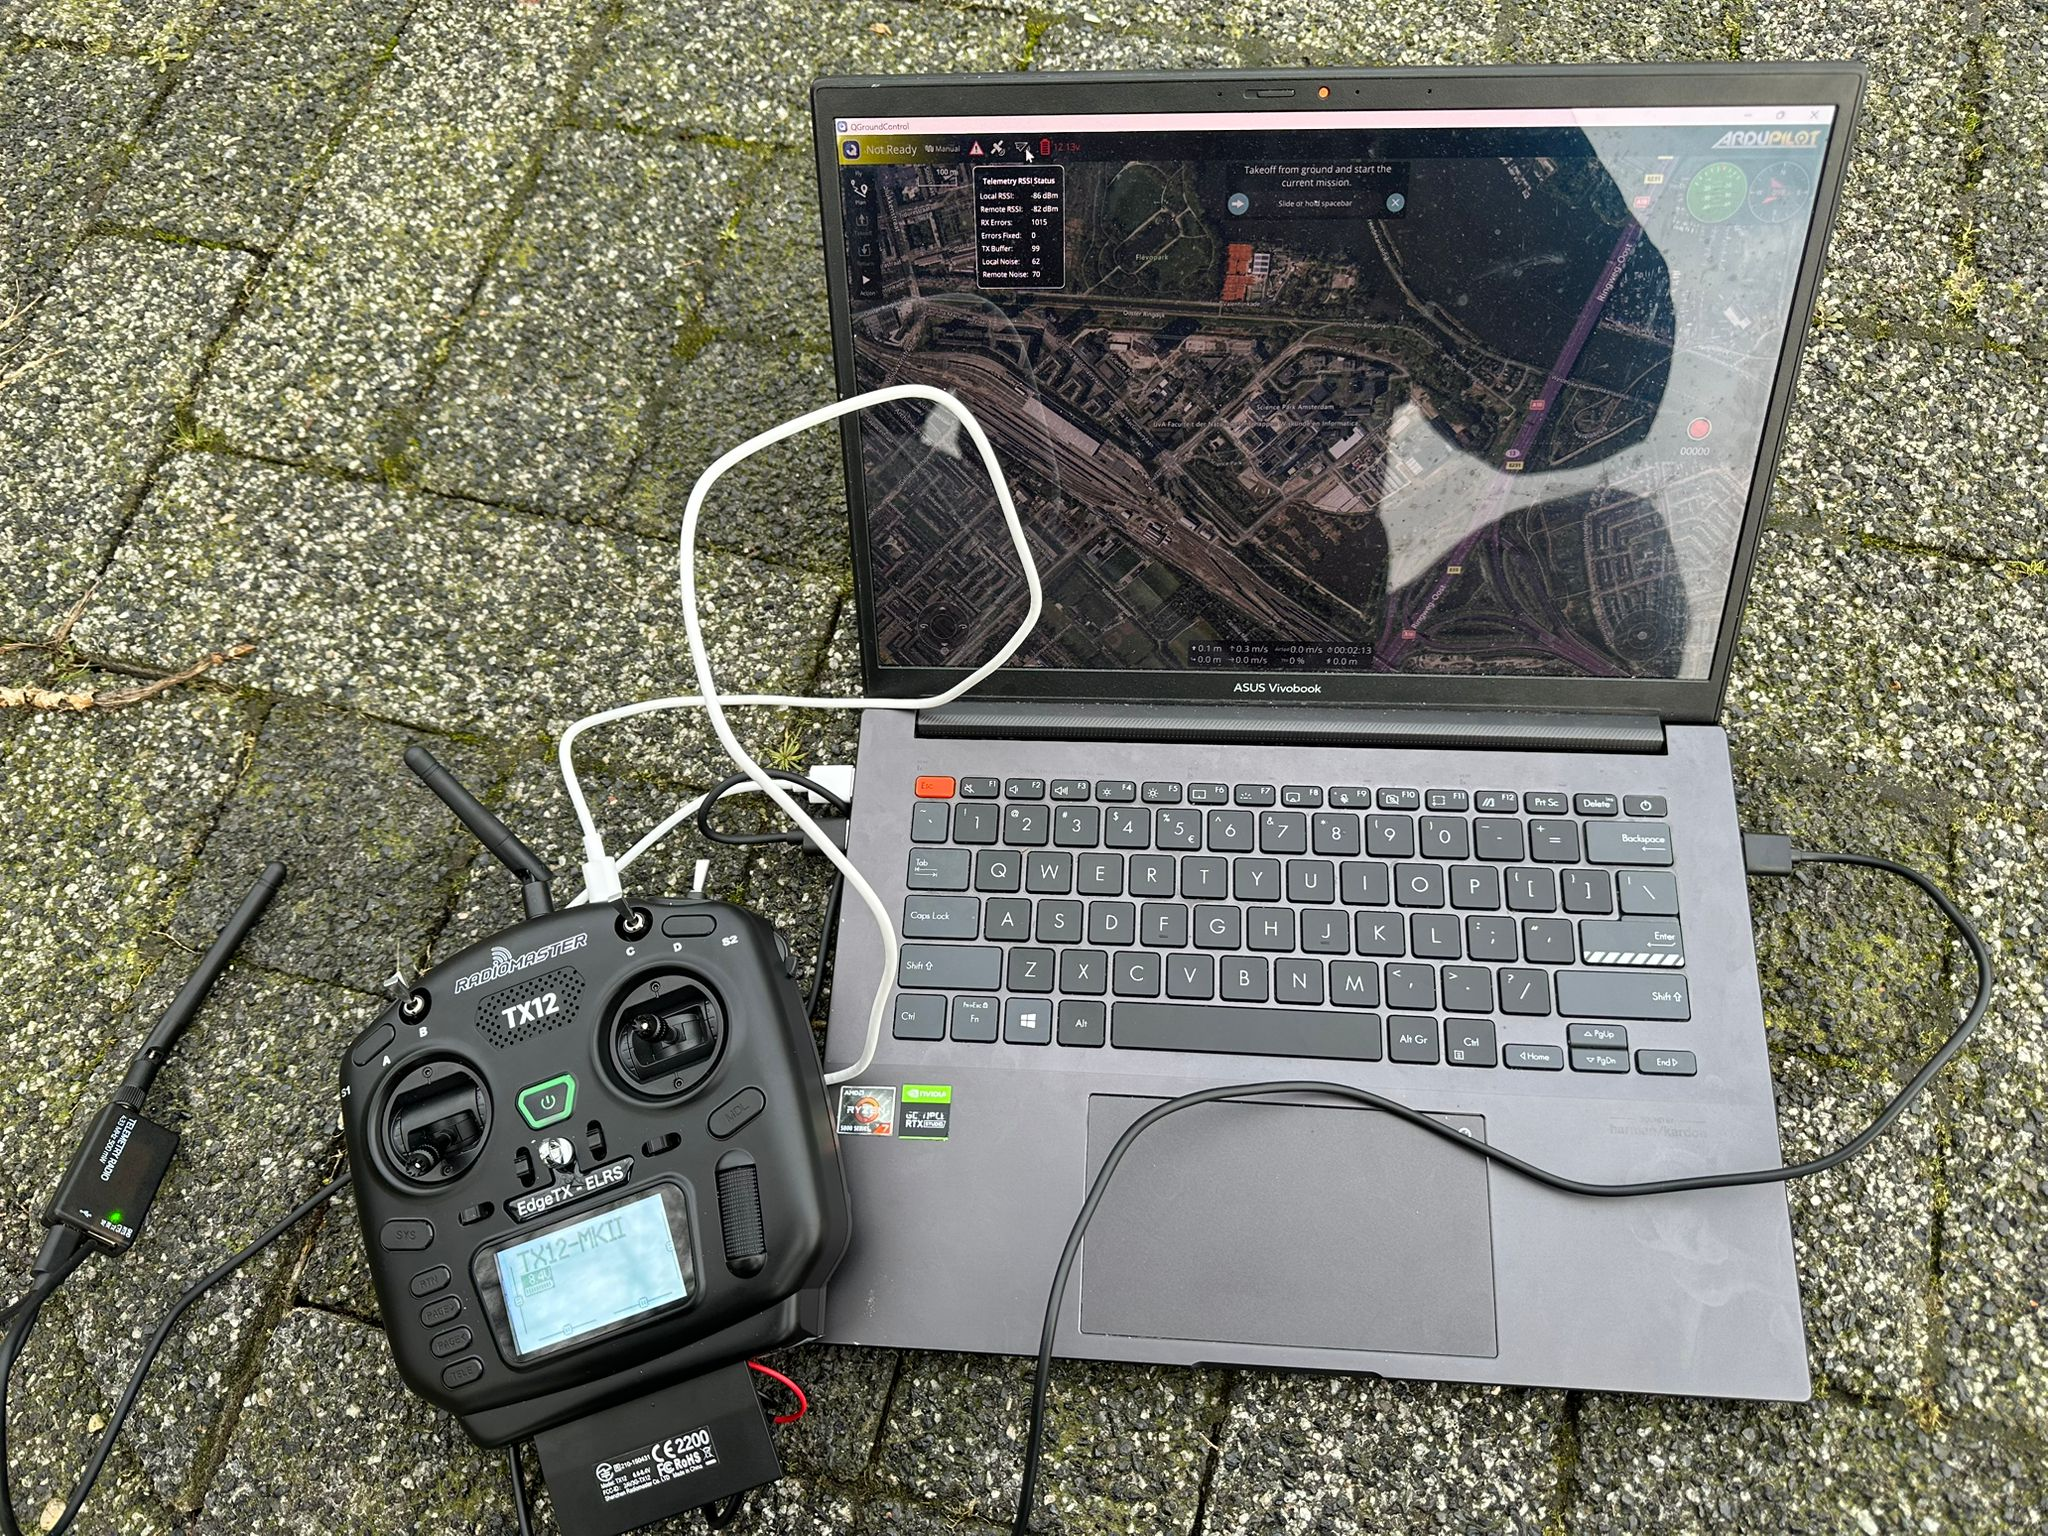
\includegraphics[width=.8\linewidth]{images/range_test2.jpg}
  \label{fig:rangesetup}
\end{subfigure}
\caption{The maximum range and testing setup}
\label{fig:range}
\end{figure}